
\chapter{Segmentation Algorithms}
\label{appendix:algorithms}

\section{Penumbra and Umbra Extraction}
The \textit{Umbra} and \textit{Penumbra} are distinctly dark spots on the continuum. When the photosphere has an abnormally high magnetic field, heat is trapped beneath the surface. The lower temperature surface ensures a lower intensity, which appears as a black or grey ``sunspot" on the surface of the sun. An umbra will sometimes have an accompanying penumbra, where the continuum shows a secondary low intensity. The penumbra is seen as a visually less dark region of the active region, but still distinct from the rest of the surface. We find Umbras and Penumbras using mathematical morphology and adaptive thresholding. These distinct regions are shown visually in figure \ref{fig:binarythresh}.

First, we extract the Umbra and Penumbra in the same algorithm. This is because the Umbra and Penumbra are very closely tied to one another. A few high level axioms guide our thinking. First, Umbra and Penumbra are darker \textit{than their surroundings}, but regions further from an Umbra may be just as dark. Therefore, rather than threshold the image as a whole, we use a localized adaptive filter that thresholds the image using localized grids. Second, a group of ``dark" pixels (low intensity) can either be unimodal (only an Umbra) or bimodal (an Umbra with an accompanying Penumbra). 

The algorithm to extract Umbras and Penumbras is shown in \ref{alg:umpum}:

\begin{enumerate}
    \item First, (lines 3-6) we bound the continuum intensity from 0 to 255. The absolute magnitude of the continuum shouldn't matter because an Umbra and Penumbra is simply a darkened region compared to their surroundings. A binary adaptive threshold \cite{scikit} takes into account that there may be shadows or dark regions in the image that are not necessarily Umbras or Penumbras. For example, in figure \ref{fig:binarythresh}, the right side of the original continuum is darkened due to a shadow, which could interfere with a global threshold. The binary adaptive threshold only considers localized kernels (in this case, we restrict the filter to a 5x5 kernel, which is chosen through experimentation, but is a parameter the user can adjust if they see fit). Each threshold is the weighted mean of the local neighborhood. After we threshold, this leaves us with a binary array showing regions that are greater than (false) or less than the adaptive threshold value (true). The output of this step is shown in figure \ref{fig:binarythresh}. Now, this whole region is set equal to the Umbra:
    
    $$Umbra \gets binaryAdaptive(C)$$
    
    and in step two, we will subtract the Penumbra from the previously defined Umbra:
    
    $$Umbra \gets Umbra \cap \neg Penumbra$$
    
\begin{figure}[h]
\centering
\begin{subfigure}[b]{.45\textwidth}
  \centering
  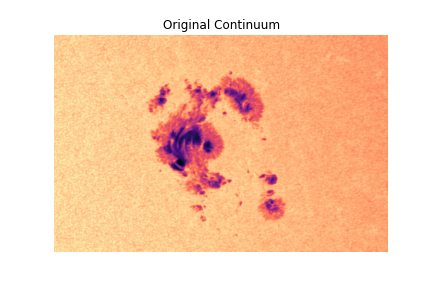
\includegraphics[width=.8\linewidth]{ThesisFilePkg/figures/data/cont_original.png}
  \caption{Original continuum intensity}
  \label{fig:binarythreshorig}
\end{subfigure}%
\quad
\begin{subfigure}[b]{.45\textwidth}
  \centering
  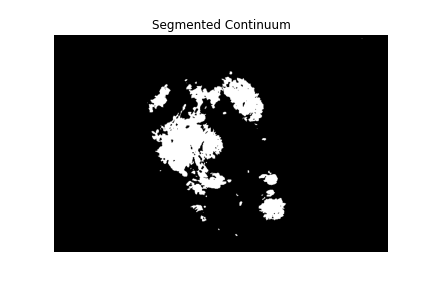
\includegraphics[width=.8\linewidth]{ThesisFilePkg/figures/data/segments.png}
  \caption{After a binary adaptive filter to \ref{fig:binarythreshorig} \cite{scikit}}
  \label{fig:binarythreshafter}
\end{subfigure}
\caption{The result of applying an adaptive binary filter to the original continuum intensity of harpnumber 7115}
\label{fig:binarythresh}
\end{figure}
    
    
    \item Second, we group all the pixels that are touching adjacently or diagonally (lines 9 - 20) and filter out groups of pixels that couldn't be considered Penumbras. This is a three-fold process. First, (lines 13-15) we remove groups that are less than 10 pixels in area. The next two filters are only to speed up computation. We then remove all clusters less than 1\% of the size of the largest cluster (lines 16-18) for the same reason we removed small clusters. Finally, of the remaining groups, we keep the largest six clusters (line 20) (at this point, this step usually doesn't filter out many groups unless the active region is noticeably large and fragmented). 
    
    
\begin{figure}[h]
\centering
\begin{subfigure}[b]{.45\textwidth}
  \centering
  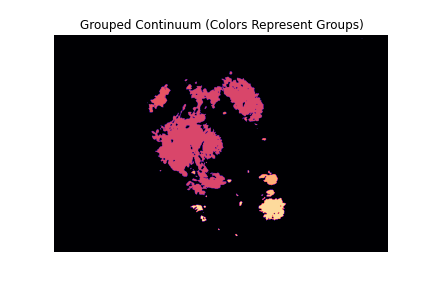
\includegraphics[width=.8\linewidth]{ThesisFilePkg/figures/data/segments_grouped.png}
  \caption{Grouped continuum. Different colors represent different groups}
  \label{fig:grouped}
\end{subfigure}%
\quad
\begin{subfigure}[b]{.45\textwidth}
  \centering
  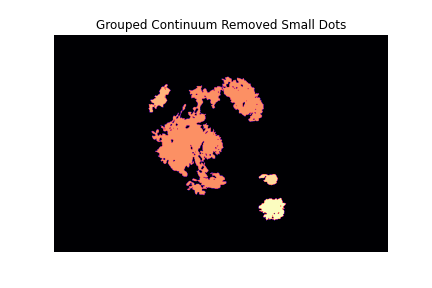
\includegraphics[width=.8\linewidth]{ThesisFilePkg/figures/data/segments_grouped_filtered.png}
  \caption{Grouped continuum after removing small pixel groups and taking the 6 largest from \ref{fig:grouped}}
  \label{fig:groupedfiltered}
\end{subfigure}
\caption{The result of grouping then filtering the active region previously segmented in figure \ref{fig:binarythresh}. It's important to note that from \ref{fig:grouped} to \ref{fig:groupedfiltered}, the Umbra segment maintains all the filtered pores. That is, we only group regions so we can find Penumbras and we assume Penumbras aren't found in these filtered groups.}
\label{fig:binarythresh}
\end{figure}
    
    
    \item Finally, we run through all clusters and determine if they are unimodal (just an Umbra) or bimodal (Penumbra and Umbra). Through experimentation, a value of 21000 is chosen as a benchmark for Umbra / Penumbra difference. That is, if the maximum minus the minimum pixel value was greater than 21000, then the region is bimodal, otherwise, it is unimodal. This number was taken by manually selecting 125 unimodal and bimodal active region images (by eye). If the sub region ($g$) is bimodal, we split it into two subsets with a threshold chosen to be halfway between the maximum and minimum pixel values (line 33). The Penumbra is all the pixels above this value. This Penumbra (as previously mentioned) is subtracted from the Umbra. Otherwise, there is no other work to be done. These segmentation parameters (21000 and halfway between the maximum and minimum) can be adjusted by the user, but sacrifices for computational effectiveness and efficiency had to be made for our specific application of solar flare forecasting.
    
\begin{figure}[h]
\centering
\begin{subfigure}[b]{.45\textwidth}
  \centering
  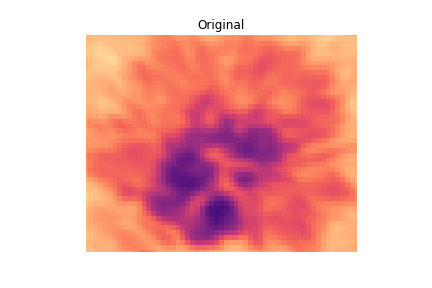
\includegraphics[width=.8\linewidth]{ThesisFilePkg/figures/data/Original_33.0.png}
  \caption{An isolated group of pixels that shows a clear Umbra and Penumbra on the continuum.}
  \label{fig:UmbraPenumbraorig}
\end{subfigure}%
\quad
\begin{subfigure}[b]{.45\textwidth}
  \centering
  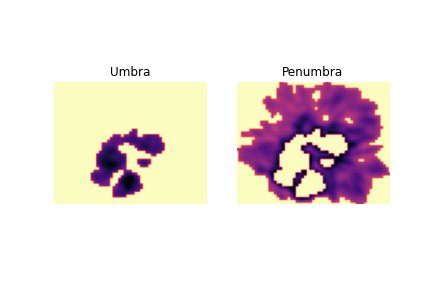
\includegraphics[width=.8\linewidth]{ThesisFilePkg/figures/data/segments_33.0.png}
  \caption{The algorithm recognizes that this subset of the continuum is bimodal, and extracts both the Penumbra and Umbra.}
  \label{fig:UmbraPenumbraseg}
\end{subfigure}
\caption{The algorithm then loops through all of the isolated groups and determines if they are unimodal or bimodal and extracts the Umbra and Penumbra from the image. \ref{fig:UmbraPenumbraorig} shows the original ``recognized" Umbra (this is a subset of the original continuum, which is found in the bottom right corner of the large darkened spot), then \ref{fig:UmbraPenumbraseg} shows the algorithm's determination of Penumbra and Umbra segments. Notice that, as expected, the Penumbra surrounds the Umbra and hugs the edges. Of course, the Umbra in \ref{fig:UmbraPenumbraseg} isn't used, it is only the Penumbra that is eventually subtracted from the Umbra because both sections are included in the original binary mask}
\label{fig:binarythresh}
\end{figure}
    
    
\end{enumerate}


\begin{algorithm}
\caption{Umbra and Penumbra Segmentation (\textit{ActiveRegion.assert\_Umbra\_Penumbra()}) }\label{alg:umpum}

\begin{algorithmic}[1]
    \State
    \State \textbf{\textit{/* Step one: Pre-process and threshold the continuum */}}
    \State $C \gets$ Continuum
    \State $C \gets \frac{C - min(C)}{max(C)} \times 255$ \Comment{Bound C by 0 and 255}
    \State $Mask \gets C < localAdaptiveThreshold(C, 5)$ \Comment{Use a square kernel of size 5x5 in the adaptive threshold} 
    \State $Umbra \gets Mask$ \Comment{The Umbra is originally all the pixels from the threshold}
    
    \State
    \State $G \gets groupPixels(Mask)$ \Comment{Group pixels that are adjacent or diagonal}
    
    \State 
    \State \textbf{\textit{/* Step two: Filter invalid groups of pixels */}}
    \For{$g \in G$}
        \If{$size(g) < 10$ pixels}
            \State $G.remove(g)$
        \EndIf
        \If{$size(g) < 0.1 * largest(G)$}
            \State $G.remove(g)$
        \EndIf
    \EndFor
   
    \State $G \gets $ Largest 6 $g \in G$ \Comment{Take only the largest 6 groups (or less)}
    
    \State
    \State \textbf{\textit{/* Step three: For each group $g$, check if it's only Umbra or Penumbra + Umbra */}}
    \State Penumbra $\gets$ Fully false $n \times m$ boolean mask
    \State 
    \For{$g \in G$}
        \State
        \State \textbf{\textit{/* Take the maximum and minimum of the continuum (not bounded) restricted to the subdomain g*/}}
        \State $Max \gets max(Continuum|_g)$ 
        \State $Min \gets min(Continuum|_g)$
        \State 
        \If{$Max - Min > 21000$} \Comment{Umbra and Penumbra}
            \State $t \gets \frac{Max - Min}{2} + Min$
            \State $Penumbra \gets Penumbra \cup ((Continuum > t) \cap g)$
        \EndIf
    \EndFor
    
    \State
    \State $Umbra \gets Umbra \cap \neg Penumbra$
    \State \textbf{Return} $Umbra, Penumbra$ 
\end{algorithmic}
\end{algorithm}


Finally, we are left with two binary masks, the Umbra and Penumbra extracted from the continuum. This is shown in figure \ref{fig:UmbraPenumbrafinal}.


\begin{figure}[h]
    \centering
    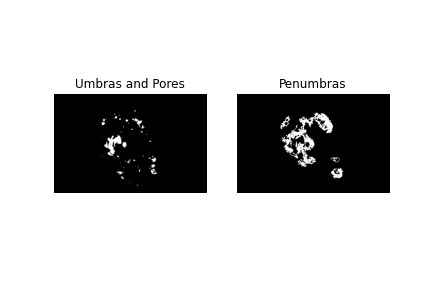
\includegraphics[width=0.7\linewidth]{ThesisFilePkg/figures/data/umbra_penumbra.png}
    \caption{The end product of the segmentation of the Umbra and Penumbra. The left shows the ``Umbra" segment (we call this the Umbra in our dataset, but it really consists of both Umbras and darkened Pores). The left shows the Penumbra segment of the continuum}
    \label{fig:UmbraPenumbrafinal}
\end{figure}

\section{Neutral Line Extraction}

The \textit{Neutral Line} is defined as a continuous subset of an active region such that the line of sight magnetic flux is (theoretically) $0\frac{Mx}{cm^2}$ and the gradient from positive to negative line of sight magnetic flux is relatively high \footnote{In this paper we use a fixed threshold and only include magnetic inversion of the active region where the absolute value of pixels is greater than $150 \frac{Mx}{cm^2}$, a value chosen by Schrijver \cite{schrijver}}. Solar flares occur frequently in these polarity inversion regions with a high magnetic field gradient. \cite{Properties2} show that the length of the neutral line with horizontal shear greater than $80^o$ performed well in a one variable discriminant analysis. This suggests that automatically detecting the neutral lines or regions of high magnetic polarity and polarity inversion could offer more information for solar physics research, flare forecasting methods, and other applications.

The Neutral Line can be extracted in it's own algorithm, which is much simpler and uses a threshold followed by a binary dilation. The algorithm to extract Neutral Lines is shown in \ref{alg:NL}:

First, we lower threshold by the absolute value of the line of sight magnetogram. We use a threshold value of $150 \frac{Mx}{cm^2}$. This leads to two disjoint subsets of the magnetic field showing highly positive and highly negative regions in figure \ref{fig:nlposneg}.


\begin{figure}[h]
    \centering
    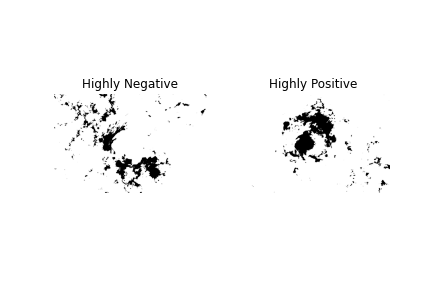
\includegraphics[width=0.5\linewidth]{ThesisFilePkg/figures/data/posneg.png}
    \caption{The result of lower thresholding the original line of sight magnetic field above and below by 150 and -150 $\frac{Mx}{cm^2}$ respectively.}
    \label{fig:nlposneg}
\end{figure}

Clearly, these two subsets are disjoint as a pixel can't be both positive and negative at the same time; but when we dilate the image, the original segments expand slightly (by 5 pixels to be exact, which is an arbitrary number that can be adjusted by the user) shown in figure \ref{fig:nldilated}. This is done in lines 7-8.

\begin{figure}[h]
    \centering
    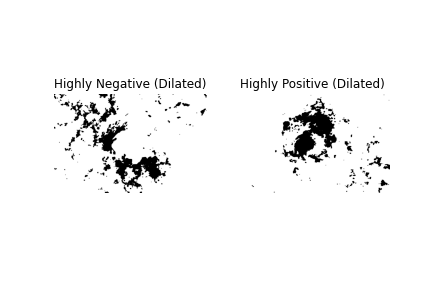
\includegraphics[width=0.5\linewidth]{ThesisFilePkg/figures/data/dilated.png}
    \caption{The result of dilating figure \ref{fig:nlposneg}. Although similar, these subsets are slightly expanded (by 5 pixels)}
    \label{fig:nldilated}
\end{figure}

By taking the intersection of these two binary dilations (line 11), we find strips of magnetic flux that rapidly change from positive to negative. Just like the Umbra and Penumbra algorithm, we group pixels and filter them, then return the union of all groups as the Neutral Line segment (lines 13-27). This is shown graphically in figure \ref{fig:nlfinal}, and is the final Neutral Line segment used in our data set.


\begin{figure}[h]
    \centering
    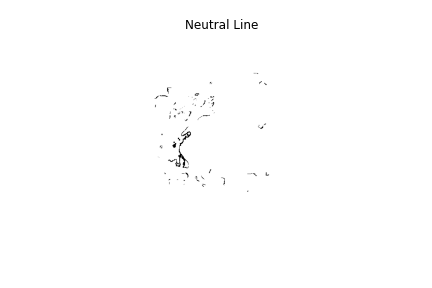
\includegraphics[width=0.7\linewidth]{ThesisFilePkg/figures/data/neutralline.png}
    \caption{The result of intersecting figure \ref{fig:nldilated}, leading to the final Neutral Line.}
    \label{fig:nlfinal}
\end{figure}


\begin{algorithm}
\caption{Neutral Line Segmentation Algorithm (\textit{ActiveRegion.assert\_neutral\_lines(radius ($r$), threshold ($t$))})}\label{alg:nl}
\label{alg:NL}

\begin{algorithmic}[1]

\State
\State \textbf{\textit{/* r is the radius of the kernel used for dilation */}}
\Require $0 < r < min(m,n)$ \Comment{where our image is of size $m\times n$}
\State
\State \textbf{\textit{/* t is the initial threshold value (chosen to be 150 $\frac{Mx}{cm^2}$)}}
\Require $0 < t$

\State
\State \textbf{\textit{/* Bz is the line of sight magnetic field array */}}
\State $mask^{+} \gets$ binaryDilation(Bz $> t$, square($r$)) \Comment{Dilate Positive pixels with an $r \times r$ square kernel}
\State $mask^{-} \gets$ binaryDilation(Bz $< -t$, square($r$)) \Comment{Dilate Negative pixels with an $r \times r$ square kernel}

\State
\State \textbf{\textit{/* The intersection of these two dilations rapidly changes from positive to negative */}}
\State $Mask \gets mask^+ \cap mask^-$ 

\State

\State $G \gets groupPixels(Mask)$ \Comment{Group pixels that are adjacent or diagonal}

\State 
\State \textbf{\textit{/* Step two: Filter invalid groups of pixels */}}
\For{$g \in G$}
    \If{$size(g) < 10$ pixels}
        \State $G.remove(g)$
    \EndIf
    \If{$size(g) < 0.1 * largest(G)$}
        \State $G.remove(g)$
    \EndIf
\EndFor

\State
\State $G \gets $ Largest 6 $g \in G$ \Comment{Take only the largest 6 groups (or less)}
\State
\State \textbf{Return} $\cup_{\forall g \in G}g$ \Comment{The union of all subregions in $G$}
\end{algorithmic}
\end{algorithm}

The final product is a segmented magnetogram as shown in figure \ref{fig:nlfinal}. 

\section{Background Extraction}

The background is simply the negation of all of the previously defined subgroups.

$$Background \gets \neg(Umbra \cup Penumbra \cup Neutral Line)$$

The background is included to be comprehensive. We do not wish to lose out of any information from the given active region and ignoring everything else other than the Umbra, Penumbra and Neutral Line could cause a loss of information.
